% Made up for the tikra benchmark.
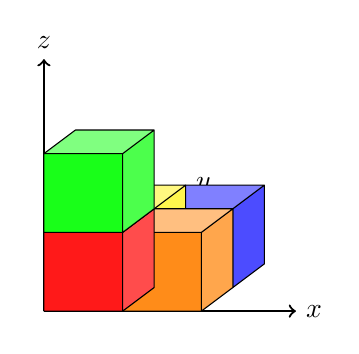
\begin{tikzpicture}[x={(1cm,0cm)}, y={(0.4cm,0.3cm)}, z={(0cm,1cm)}, line join=round]
  \draw[->, thick] (0,0,0) -- (3.2,0,0) node[right] {$x$};
  \draw[->, thick] (0,0,0) -- (0,4.5,0) node[above right] {$y$};
  \draw[->, thick] (0,0,0) -- (0,0,3.2) node[above] {$z$};
  \foreach \x/\y/\z/\c in {1/1/0/blue, 0/1/0/yellow, 1/0/0/orange, 0/0/0/red, 0/0/1/green} {
    \fill[\c!50] (\x,\y,\z+1) -- (\x+1,\y,\z+1) -- (\x+1,\y+1,\z+1) -- (\x,\y+1,\z+1) -- cycle;
    \fill[\c!70] (\x+1,\y,\z) -- (\x+1,\y+1,\z) -- (\x+1,\y+1,\z+1) -- (\x+1,\y,\z+1) -- cycle;
    \fill[\c!90] (\x,\y,\z) -- (\x+1,\y,\z) -- (\x+1,\y,\z+1) -- (\x,\y,\z+1) -- cycle;
    \draw (\x,\y,\z+1) -- (\x+1,\y,\z+1) -- (\x+1,\y+1,\z+1) -- (\x,\y+1,\z+1) -- cycle
          (\x,\y,\z) -- (\x+1,\y,\z) -- (\x+1,\y,\z+1) -- (\x,\y,\z+1) -- cycle
          (\x+1,\y,\z) -- (\x+1,\y+1,\z) -- (\x+1,\y+1,\z+1);
  }
\end{tikzpicture}
